% !Mode:: "TeX:UTF-8"
% !TeX root = SDUthesistemplate.tex
%!TEX program = xelatex
%\expandafter\def\csname CTEX@spaceChar\endcsname{\hspace{1em}}

%==============================================================
% 学位类型切换方式（见 contents/titlepageinfo.tex）：
%
%   学术学位（默认/黑色）：\DegreeType{（学术学位）}
%   专业学位（红色）：     \DegreeType{\textcolor{SDUred}{（专业学位）}}
%
% 在 titlepageinfo.tex 中取消对应行的注释即可，不要修改本文件。
%==============================================================
\documentclass[single,print]{sduthesis}

% !Mode:: "TeX:UTF-8"
% titlepageinfo.tex
% 中图分类号
\fenlei{*自己查找}
% 单位代号
\DWdaihao{10422}
% 密级
\miji{公开}
% 学号
\StuNum{123456789}
% 页眉
\ThesisHeader{山东大学硕士学位论文}
\EThesisHeader{Shandong University Master Thesis}
% 论文类型（封面） 中
\CThesisType{硕~士~学~位~论~文}
% 论文类型（封面） 英
\EThesisType{Thesis for Master Degree}
% 中文标题
\Ctitle{硕士学位论文题目示例}
% 英文标题
\Etitle{An Example Title for Master Thesis}
% 作者中文名
\Cauthor{作者姓名}
% 学院
\Dpart{某某学院}

% 培养方式
\Dform{全日制}


% 学位类型（封面）：学术学位 / 专业学位（二选一，取消注释即可）
\DegreeType{（学术学位）}                % 黑色
%\DegreeType{\textcolor{SDUred}{（专业学位）}}  % 红色

% 专业中文名
\Cmajor{某某专业}
% 年级
%\Grade{xxxx级}
% 指导老师中文名
\Csuperver{指导老师~~教授}
\Ccosuperver{合作导师~~教授}
% 中文日期
\Cdate{\today}
\title{\the\Ctitle}
\author{\the\Cauthor}
\date{\the\Cdate}

\input{contents/usersettings.tex}

\begin{document}

% 首页及原创性声明
\maketitlepagestatement
\cleardoublepage
% 大写罗马页码
\pagenumbering{Roman}\setcounter{page}{1}

\cleardoublepage
% 中英文摘要
% !Mode:: "TeX:UTF-8"
%
% abstract.tex — 中英文摘要
%
% cnabstract / enabstract 环境由 sduthesis.cls 定义，
% 已自动设置好字体（宋体小四）、行距（固定20磅）、缩进（2字符）。
%

\begin{cnabstract}

这是论文的中文摘要。摘要概述研究背景、问题、方法、结果和结论，使读者快速了解论文内容。

本模板展示了山东大学硕士学位论文的常用排版格式，包括公式、表格、图片、算法、定理环境、参考文献引用等功能。用户可按需替换内容，参照格式排版。

\cnkeywords{关键词一；关键词二；关键词三}

\end{cnabstract}

\begin{enabstract}

This is the English abstract. It summarizes the research background, problem, method, results, and conclusions of the thesis.

This template demonstrates the formatting conventions for Shandong University master's thesis, including equations, tables, figures, algorithms, theorem environments, and bibliography management.

\enkeywords{keyword one; keyword two; keyword three}

\end{enabstract}

% Chinese TOC
%\pagenumbering{Roman}\setcounter{page}{1}
% \begin{KeepFromToc}

\setcounter{tocdepth}{1} % 设置目录显示深度：1只显示到Section，2显示到Subsection，3显示到Subsubsection

\maketableofcontents
%\end{KeepFromToc}
%\cleardoublepage
% English TOC
\tableofengcontents
\begin{symboldescription}
	\begin{tabularx}{\textwidth}{X X}
		\(x\) & 输入变量或状态变量 \\
		\(y\) & 输出变量或目标变量 \\
		\(\hat{y}\) & 模型预测值 \\
		\(\theta\) & 模型参数 \\
		\(\mathcal{L}\) & 损失函数 \\
		\(\nabla\) & 梯度算子 \\
		\(\mathbb{E}[\cdot]\) & 数学期望 \\
		\(\mathbb{P}\) & 概率测度 \\
		\(\mathcal{N}(\mu, \Sigma)\) & 高斯分布 \\
		\(\sigma(\cdot)\) & 激活函数或标准差 \\
		\(\alpha\) & 学习率 \\
		\(\lambda\) & 正则化系数 \\
		\(\mathbb{R}^n\) & \(n\) 维欧氏空间 \\
		\(f_\theta\) & 参数为 \(\theta\) 的模型函数 \\
	\end{tabularx}
\end{symboldescription}

\newpage


% 阿拉伯数字页码
\pagenumbering{arabic}\setcounter{page}{1}

% 正文
% \input{contents/body.tex}
% !Mode:: "TeX:UTF-8"
%
% 第一章：绪论
%
% 本节展示的用法：
%   - 公式（equation 环境）
%   - 定理环境（definition / theorem / lemma / corollary / remark）
%   - 参考文献引用（\cite{}）
%

\chapter{绪论}
\echapter{Introduction}
\label{chap:introduction}

本章介绍论文的研究背景、相关工作以及组织结构，并展示模板支持的各类排版环境。

\section{研究背景}
\esection{Research Background}
\label{sec:background}

随着科学技术的不断发展，数学建模方法在众多领域得到了广泛应用。相关研究在理论和实践层面都取得了重要进展\cite{ho2020denoising}。

\subsection{问题描述}
\label{subsec:problem}

设 \(X\) 为一随机变量，其期望值定义为
\begin{equation}
\mathbb{E}[X] = \int_{\Omega} X(\omega) \,\mathrm{d}\mathbb{P}(\omega),
\label{eq:expectation}
\end{equation}
方差定义为 \(\mathrm{Var}(X) = \mathbb{E}[(X - \mathbb{E}[X])^2]\)。

\subsection{基本定义}
\label{subsec:definitions}

\begin{definition}
设 \((\Omega, \mathcal{F}, \mathbb{P})\) 为一概率空间。称 \(X: \Omega \to \mathbb{R}\) 为随机变量，若对任意 \(a \in \mathbb{R}\)，有 \(\{\omega: X(\omega) \leq a\} \in \mathcal{F}\)。
\end{definition}

\begin{theorem}[大数定律]
设 \(\{X_n\}\) 为独立同分布随机变量，\(\mathbb{E}[X_1] = \mu\)，则
\begin{equation}
\frac{1}{n}\sum_{i=1}^n X_i \xrightarrow{\text{a.s.}} \mu.
\label{eq:lln}
\end{equation}
\end{theorem}

\begin{lemma}
对于任意随机变量 \(X, Y\)，有 \(\mathbb{E}[(X+Y)^2] \leq 2\mathbb{E}[X^2] + 2\mathbb{E}[Y^2]\)。
\end{lemma}

\begin{corollary}
由引理可得 \(L^2\) 空间中的三角不等式。
\end{corollary}

\begin{remark}
以上结论在后续章节中会反复使用。
\end{remark}

\section{文章组织}
\esection{Thesis Organization}

本文的结构安排如下：第\ref{chap:preliminaries}章介绍预备知识；第\ref{chap:method}章详述方法；第\ref{chap:experiments}章展示实验；最后总结全文。

% !Mode:: "TeX:UTF-8"
%
% 第二章：预备知识
%
% 本节展示的用法：
%   - 算法环境（algorithm2e）
%   - 表格（table + tabular + booktabs）
%   - 列表（itemize）
%   - 简单公式
%

\chapter{预备知识}
\echapter{Preliminaries}
\label{chap:preliminaries}

本章介绍后续所需的基础知识，包括优化方法和矩阵运算等。

\section{优化方法}
\esection{Optimization Methods}
\label{sec:optimization}

\subsection{梯度下降法}
\label{subsec:gd}

考虑无约束优化问题
\begin{equation}
\min_{x \in \mathbb{R}^n} f(x),
\label{eq:opt_prob}
\end{equation}
梯度下降的迭代格式为 \(x_{k+1} = x_k - \alpha_k \nabla f(x_k)\)。

常用的优化方法包括：
\begin{itemize}
\item \textbf{梯度下降}：一阶迭代方法，收敛慢但每步计算量小。
\item \textbf{牛顿法}：利用二阶 Hessian 矩阵加速收敛。
\item \textbf{拟牛顿法}：近似 Hessian 矩阵，平衡收敛速度与计算开销。
\end{itemize}

算法\ref{alg:sgd}给出了随机梯度下降的实现流程。

\begin{algorithm}[h]
\caption{随机梯度下降（SGD）}
\label{alg:sgd}
\SetAlgoLined
\KwIn{初始参数 \(x_0\)，学习率 \(\{\alpha_k\}\)，迭代次数 \(K\)}
\KwOut{优化结果 \(x_K\)}
\For{\(k = 0\) \KwTo \(K-1\)}{
    采样小批量 \(\mathcal{B}_k\)\;
    计算梯度 \(g_k = \frac{1}{|\mathcal{B}_k|} \sum_{i \in \mathcal{B}_k} \nabla f_i(x_k)\)\;
    更新 \(x_{k+1} = x_k - \alpha_k g_k\)\;
}
\Return \(x_K\)\;
\end{algorithm}

\section{矩阵运算}
\esection{Matrix Operations}
\label{sec:matrix}

表\ref{tab:methods}对比了不同优化方法的特点。

\begin{table}[h]
\centering
\caption{不同优化方法的对比}
\label{tab:methods}
\begin{tabular}{lccc}
\toprule
方法 & 收敛速度 & 内存开销 & 实现难度 \\
\midrule
梯度下降 & 慢 & 低 & 简单 \\
牛顿法 & 快 & 高 & 中等 \\
拟牛顿法 & 较快 & 中等 & 较复杂 \\
\bottomrule
\end{tabular}
\end{table}

% !Mode:: "TeX:UTF-8"
%
% 第三章：方法
%
% 本节展示的用法：
%   - 图片插入（figure + includegraphics）
%   - 公式（equation 环境）
%   - 交叉引用（\ref{}）
%

\chapter{方法}
\echapter{Proposed Method}
\label{chap:method}

本章介绍本文提出的方法。图\ref{fig:framework}展示了整体框架。

\begin{figure}[h]
\centering
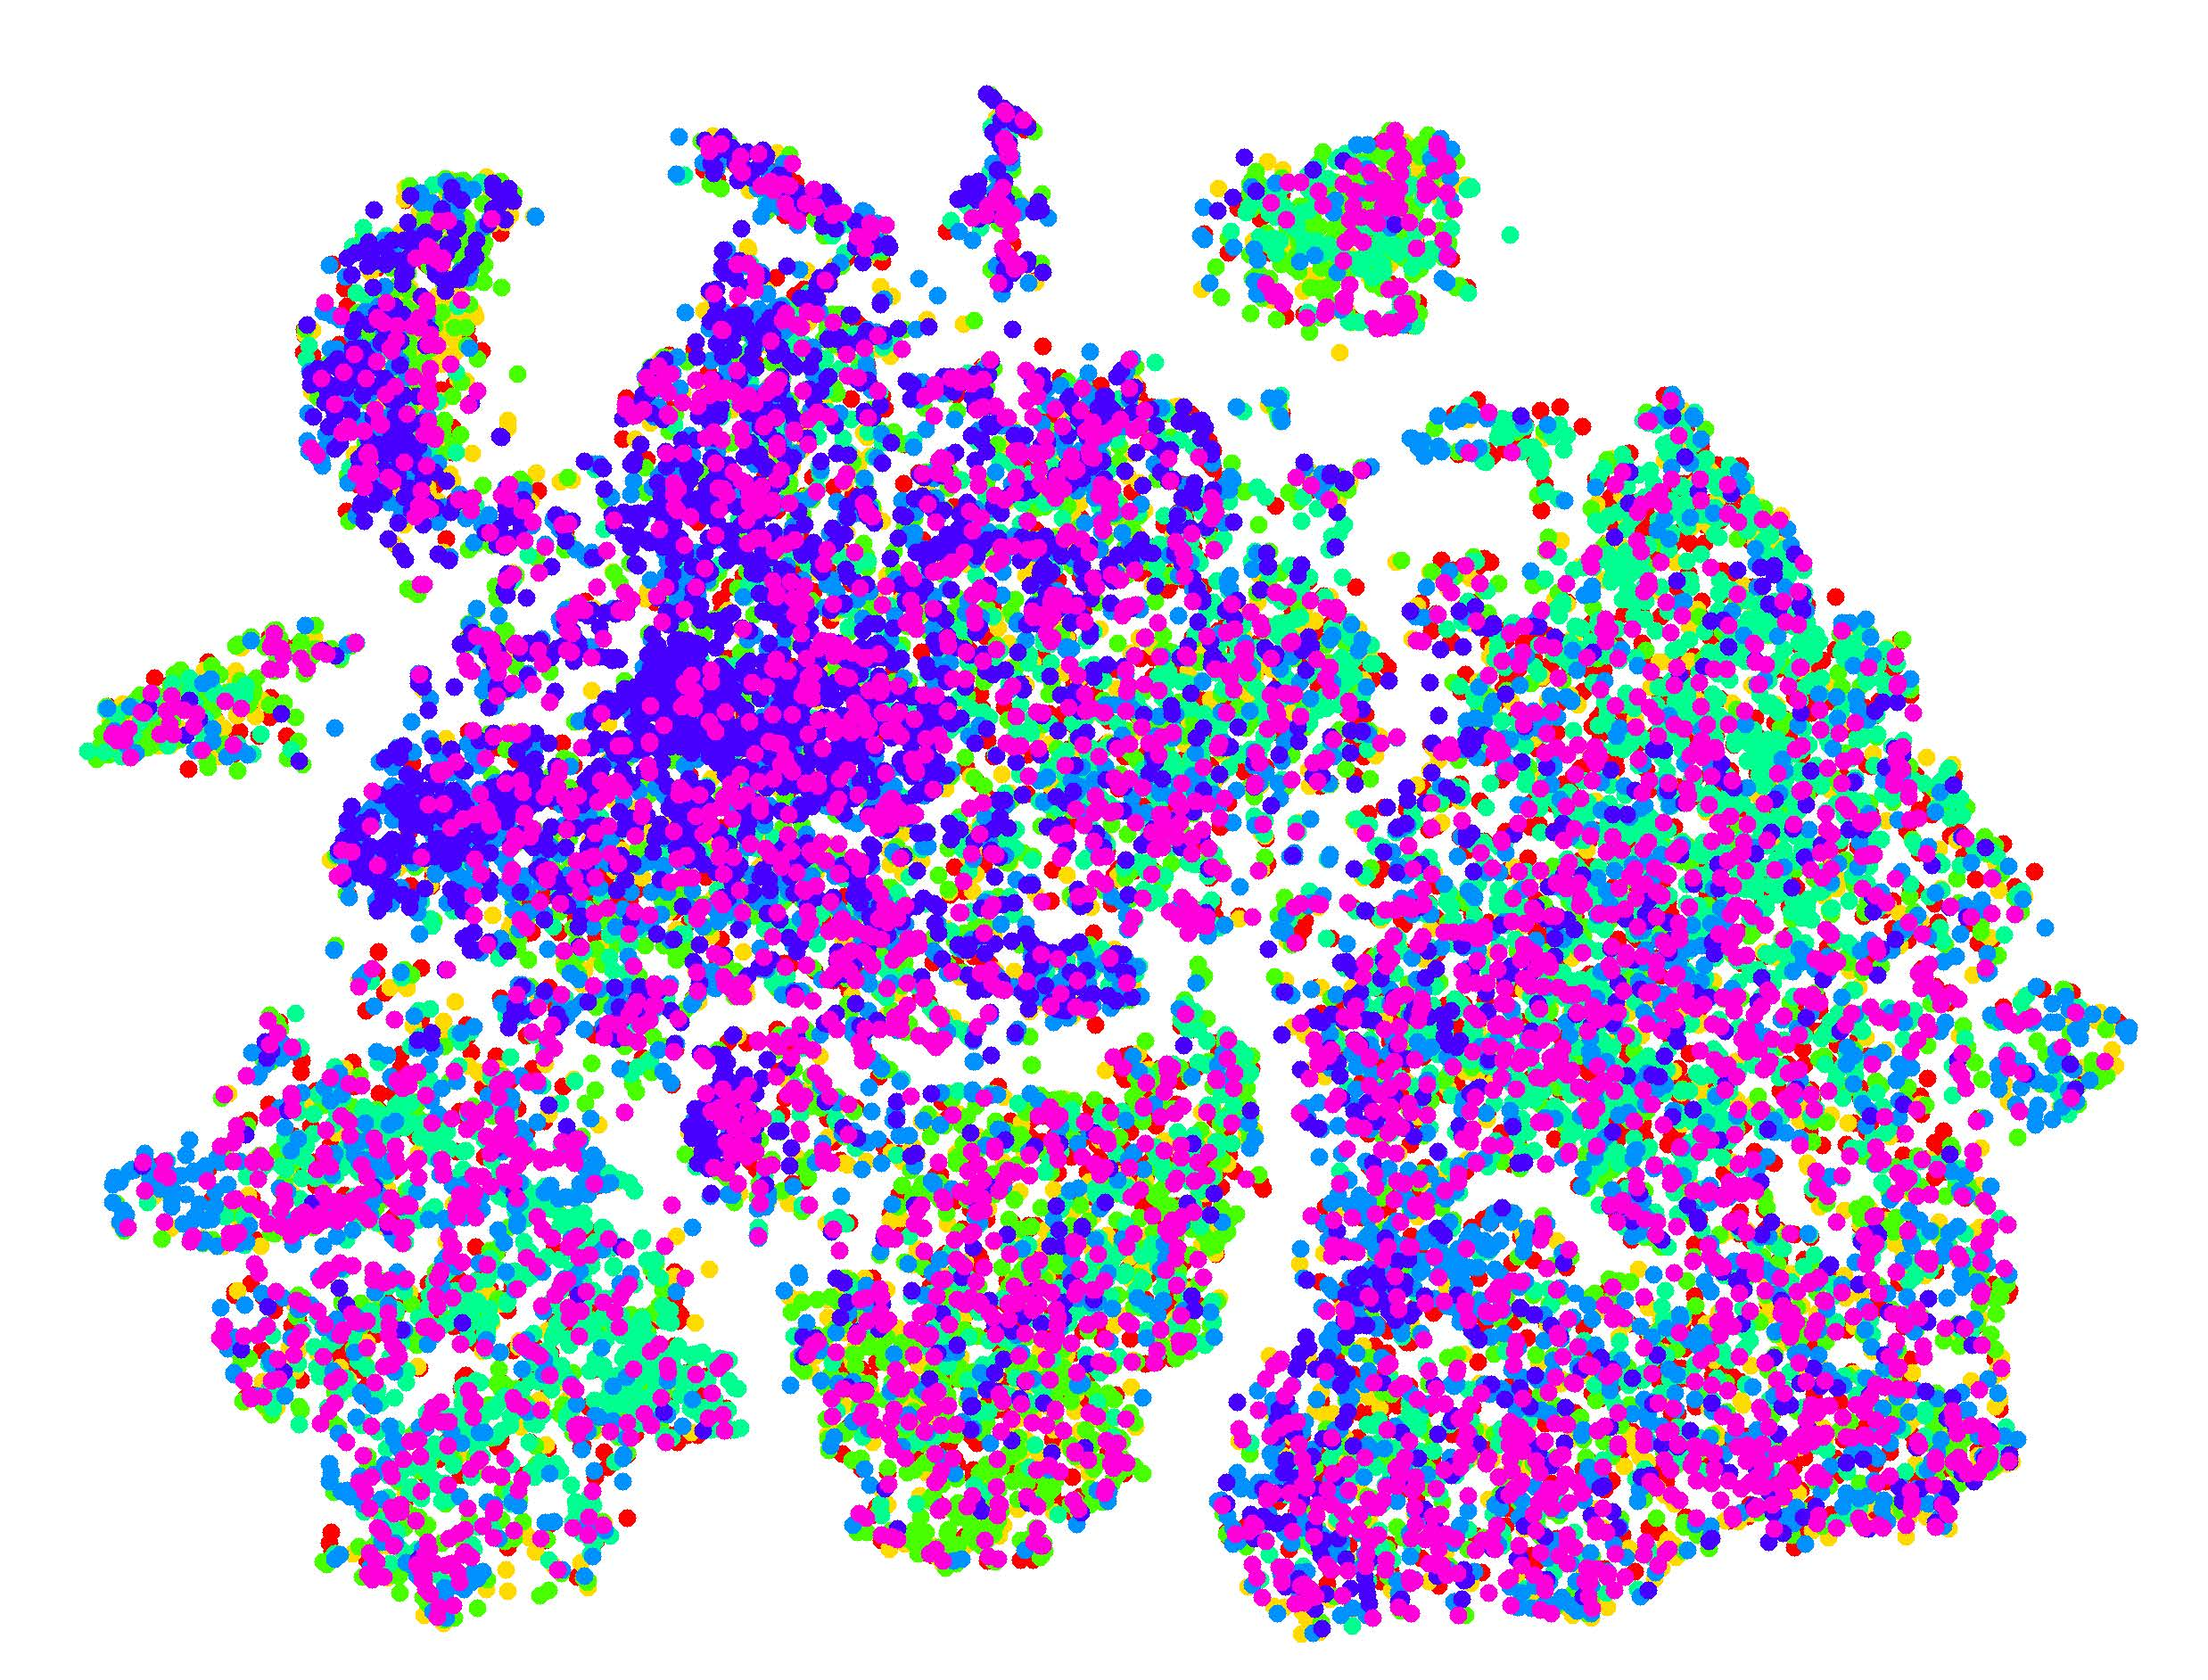
\includegraphics[width=0.6\textwidth]{figures/GIST}
\caption{方法的整体框架示意图}
\label{fig:framework}
\end{figure}

\section{模型定义}
\esection{Model Definition}
\label{sec:model_def}

设输入为 \(x \in \mathbb{R}^d\)，模型输出为
\begin{equation}
\hat{y} = f_\theta(x) = W_2 \cdot \sigma(W_1 x + b_1) + b_2,
\label{eq:model}
\end{equation}
其中 \(\theta = \{W_1, b_1, W_2, b_2\}\) 为可学习参数，\(\sigma(\cdot)\) 为激活函数。

\section{损失函数}
\esection{Loss Function}
\label{sec:loss}

模型通过最小化以下损失进行训练：
\begin{equation}
\mathcal{L}(\theta) = \frac{1}{N} \sum_{i=1}^N \ell(y_i, \hat{y}_i) + \lambda \cdot \Omega(\theta),
\label{eq:loss}
\end{equation}
其中 \(\ell\) 为任务损失（回归用 MSE，分类用交叉熵），\(\Omega\) 为正则项。

\section{训练流程}
\esection{Training Pipeline}

算法\ref{alg:training}总结了完整的训练流程，详见第\ref{chap:implementation}章。

\begin{algorithm}[h]
\caption{训练流程}
\label{alg:training}
\SetAlgoLined
\KwIn{数据集 \(\mathcal{D}\)，初始参数 \(\theta_0\)}
\KwOut{\(\theta^*\)}
\For{epoch = 1 \KwTo \(E\)}{
    \For{每个小批量 \(\mathcal{B} \subset \mathcal{D}\)}{
        \(\theta \leftarrow \theta - \alpha \nabla \mathcal{L}_{\mathcal{B}}(\theta)\)\;
    }
}
\Return \(\theta\)\;
\end{algorithm}

% !Mode:: "TeX:UTF-8"
%
% 第四章：实现细节
%
% 本节展示的用法：
%   - 多行合并表格（multirow）
%   - 子图排版（subfloat）
%   - 矩阵公式（pmatrix）
%   - 分段函数（cases）
%   - 单图插入
%

\chapter{实现细节}
\echapter{Implementation Details}
\label{chap:implementation}

本章介绍方法的具体实现细节。

\section{数据增强}
\esection{Data Augmentation}
\label{sec:augmentation}

表\ref{tab:aug}列出了使用的数据增强策略。

\begin{table}[h]
\centering
\caption{数据增强策略}
\label{tab:aug}
\begin{tabular}{lcc}
\toprule
增强方法 & 概率 & 参数说明 \\
\midrule
随机旋转 & 0.5 & \([-15^\circ, 15^\circ]\) \\
水平翻转 & 0.5 & — \\
高斯噪声 & 0.3 & \(\sigma = 0.01\) \\
\bottomrule
\end{tabular}
\end{table}

\section{网络架构}
\esection{Network Architecture}
\label{sec:arch}

表\ref{tab:arch}展示了网络结构。

\begin{table}[h]
\centering
\caption{网络架构}
\label{tab:arch}
\begin{tabular}{ccl}
\toprule
\multirow{2}{*}{特征提取}
& 卷积层 \(3\times3\) & 64 通道 \\
& 池化层 & \(2\times2\) \\
\midrule
\multirow{2}{*}{分类头}
& 全连接层 & 256 维 \\
& Softmax 输出 & 10 类 \\
\bottomrule
\end{tabular}
\end{table}

\section{可视化示例}
\esection{Visualization Examples}
\label{sec:vis}

图\ref{fig:single}为单图示例，图\ref{fig:subfigs}为子图排版示例。

\begin{figure}[h]
\centering
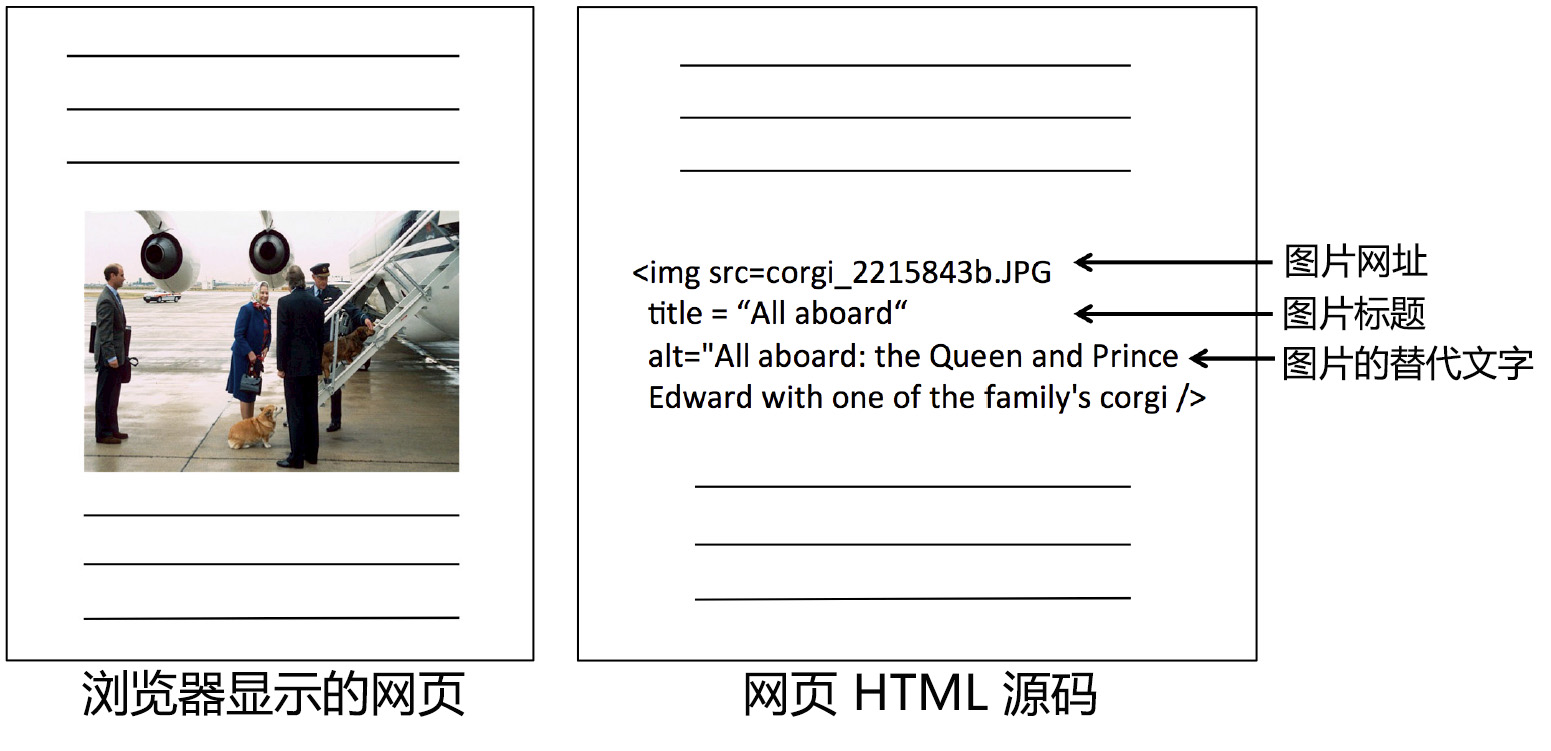
\includegraphics[width=0.5\textwidth]{figures/htmltext}
\caption{单图插入示例}
\label{fig:single}
\end{figure}

\begin{figure}[h]
\centering
\subfloat[子图一]{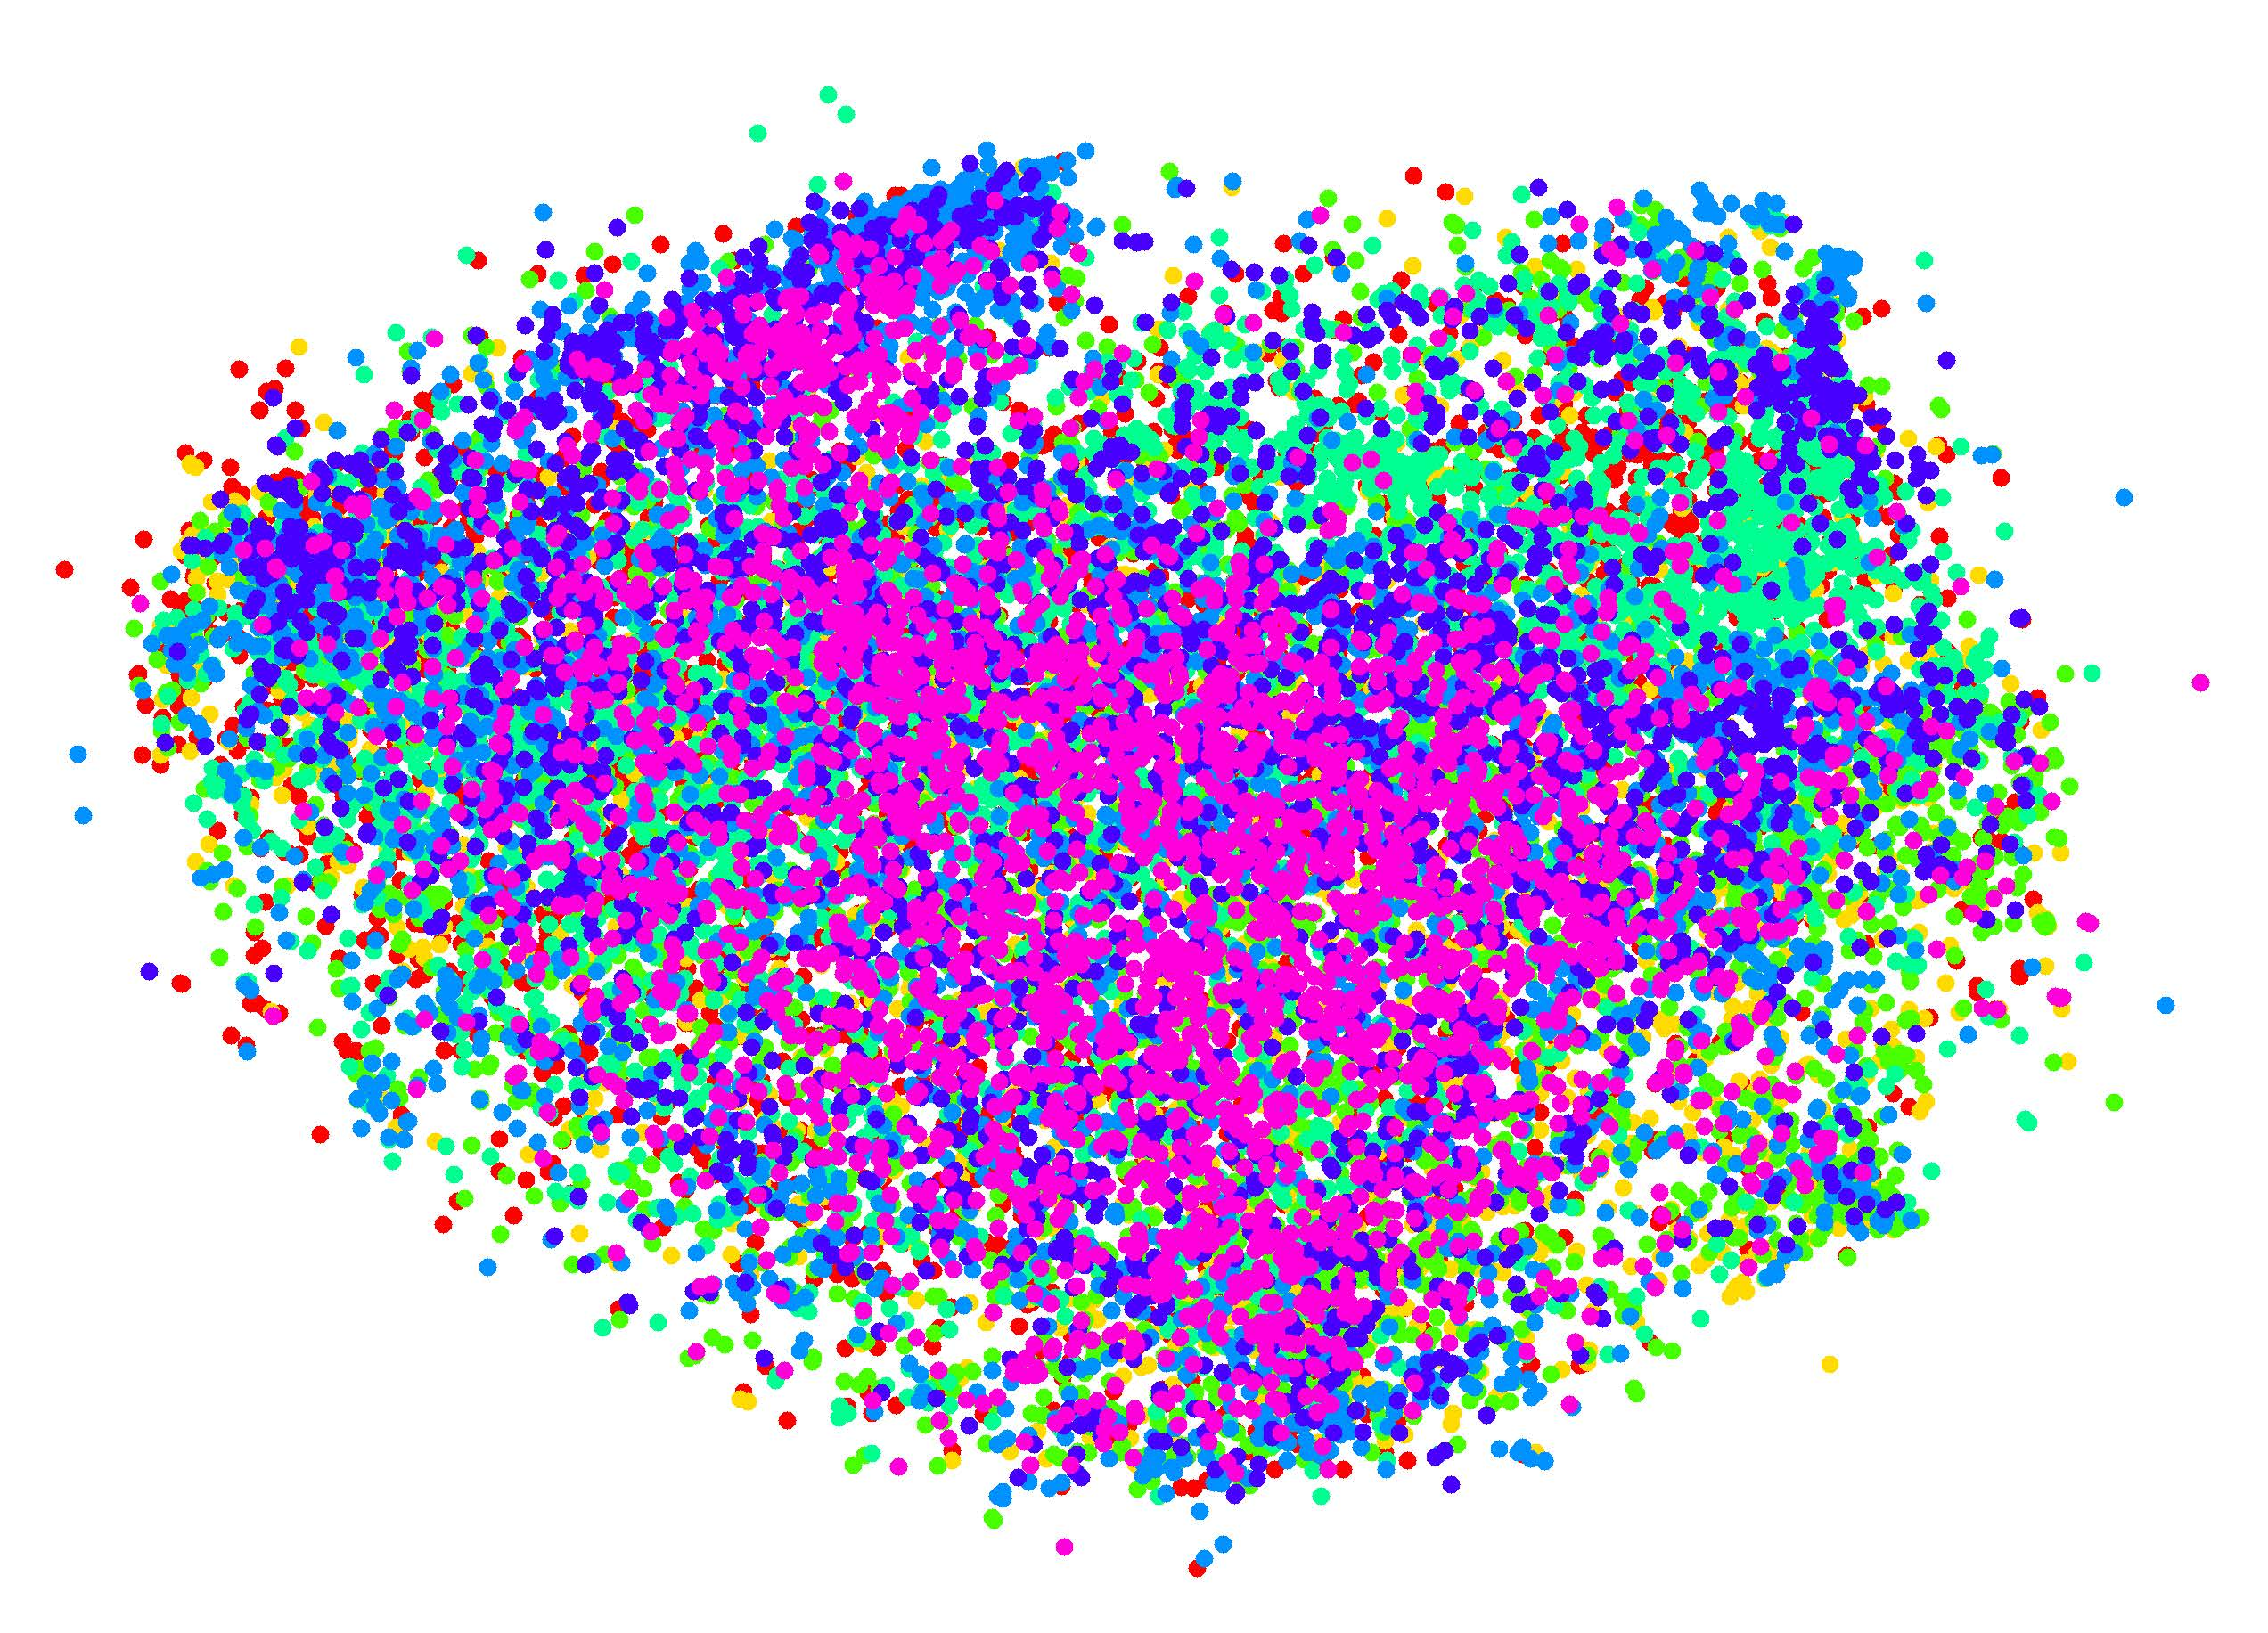
\includegraphics[width=0.28\textwidth]{figures/DECAF1}\label{fig:a}}
\qquad
\subfloat[子图二]{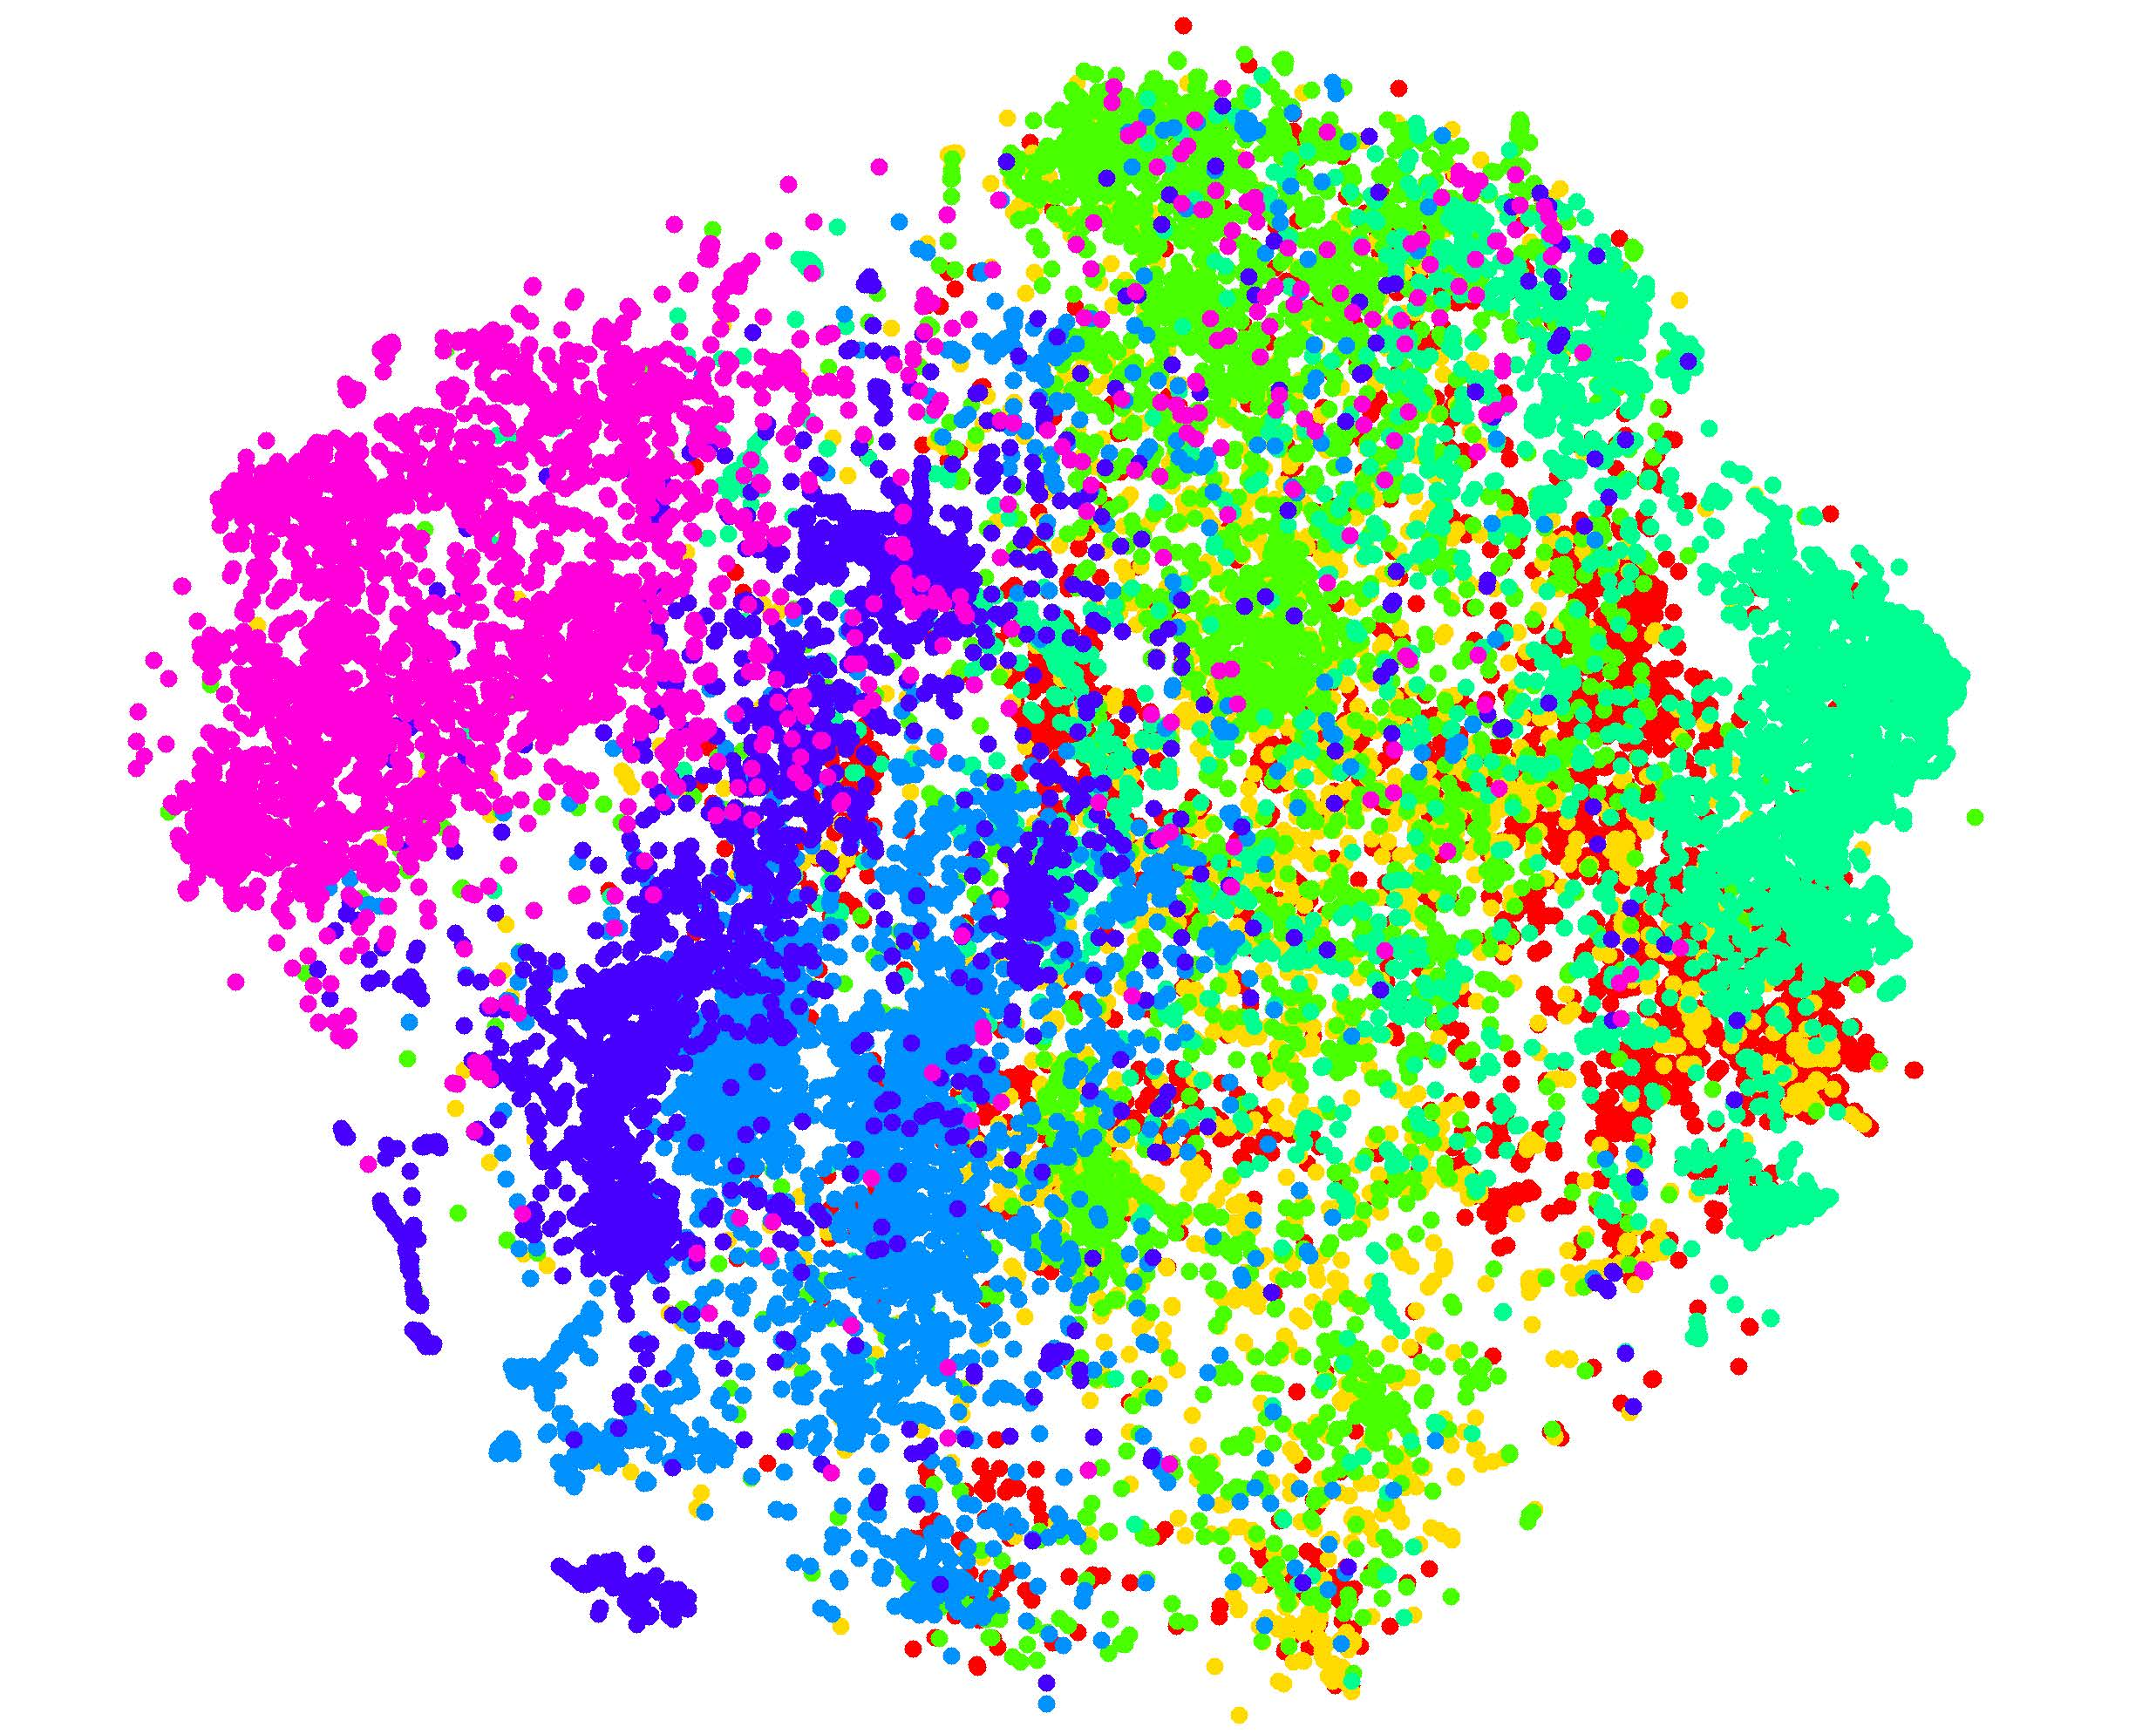
\includegraphics[width=0.28\textwidth]{figures/DECAF6}\label{fig:b}}
\caption{多子图排版示例}
\label{fig:subfigs}
\end{figure}

\section{数学公式}
\esection{Math Formulas}
\label{sec:math}

矩阵与分段函数的写法示例：
\begin{equation}
A = \begin{pmatrix}
a_{11} & a_{12} \\
a_{21} & a_{22}
\end{pmatrix},
\qquad
\frac{\partial u}{\partial t} =
\begin{cases}
\alpha \nabla^2 u, & x \in \Omega,\; t > 0,\\
u_0(x), & t = 0.
\end{cases}
\label{eq:matrix_cases}
\end{equation}

% !Mode:: "TeX:UTF-8"
%
% 第五章：实验
%
% 本节展示的用法：
%   - 结果表格（三线表 + 加粗突出）
%   - 图片插入
%   - 交叉引用（\ref{} 引用图表）
%   - 段落文字
%

\chapter{实验评估与结果分析}
\echapter{Experimental Evaluation and Analysis}
\label{chap:experiments}

本章通过实验评估所提方法的有效性。

\section{实验设置}
\esection{Experimental Setup}
\label{sec:setup}

实验环境配置：Intel i7-12700K，NVIDIA RTX 3090，PyTorch 2.0。评价指标包括准确率（Accuracy）和 F1 分数。

\section{主要结果}
\esection{Main Results}
\label{sec:main_results}

表\ref{tab:results}展示了与基线方法的对比结果。

\begin{table}[htbp]
\centering
\caption{与基线方法的性能对比}
\label{tab:results}
\begin{tabular}{lccc}
\toprule
方法 & 准确率 (\%) & F1 分数 & 训练时间 (min) \\
\midrule
基线 A & 85.32 & 0.842 & 45 \\
基线 B & 87.15 & 0.861 & 52 \\
\textbf{本文方法} & \textbf{91.27} & \textbf{0.905} & 50 \\
\bottomrule
\end{tabular}
\end{table}

\section{收敛性分析}
\esection{Convergence Analysis}
\label{sec:convergence}

图\ref{fig:convergence}展示了训练过程中的损失曲线，模型能够快速稳定收敛。

\begin{figure}[htbp]
\centering
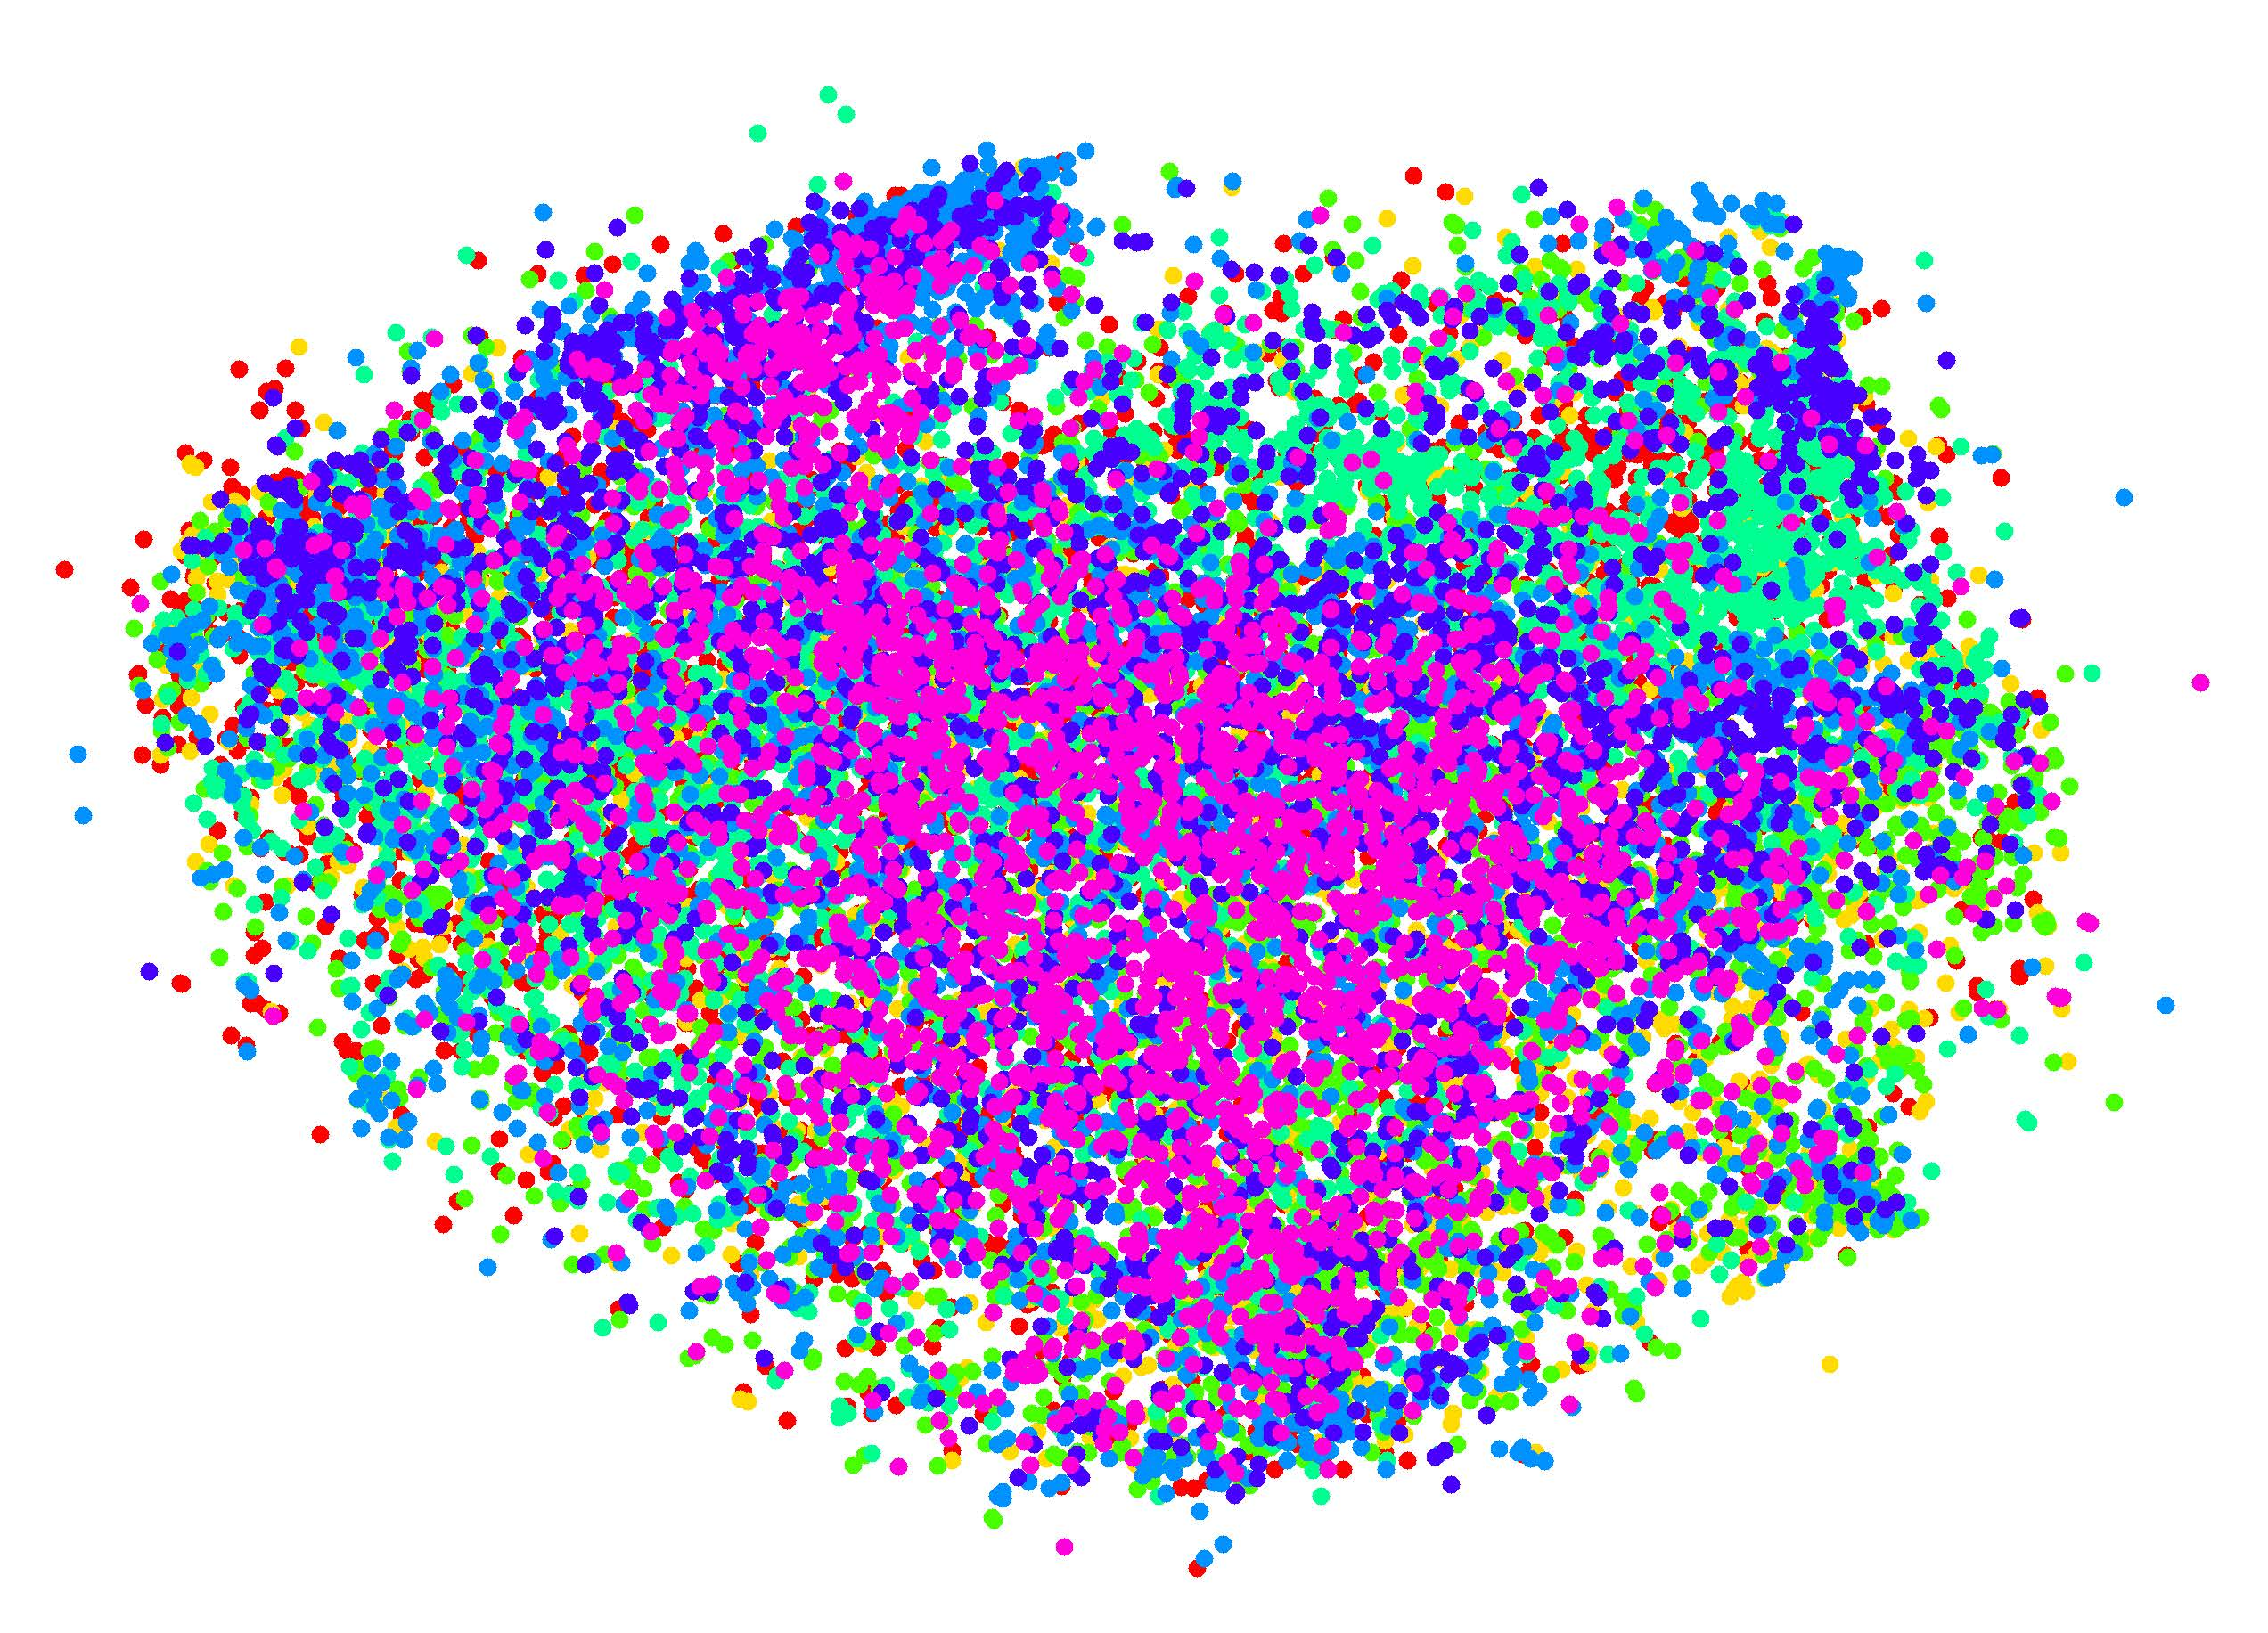
\includegraphics[width=0.5\textwidth]{figures/DECAF1}
\caption{训练损失收敛曲线}
\label{fig:convergence}
\end{figure}

\section{消融实验}
\esection{Ablation Study}
\label{sec:ablation}

表\ref{tab:ablation}的消融实验表明，各个模块对最终性能均有显著贡献。

\begin{table}[htbp]
\centering
\caption{消融实验结果}
\label{tab:ablation}
\begin{tabular}{lccc}
\toprule
配置 & 准确率 (\%) & F1 分数 \\
\midrule
仅基线 & 82.15 & 0.803 \\
去掉模块 A & 79.32 & 0.781 \\
去掉模块 B & 71.88 & 0.702 \\
完整模型 & \textbf{91.27} & \textbf{0.905} \\
\bottomrule
\end{tabular}
\end{table}

% !Mode:: "TeX:UTF-8"
%
% conclusions.tex — 结论
%
% 使用 \chapter 命令，会生成带编号的章节。
% 如需不加编号，可将 \chapter 改为 \chapter* 并手动添加目录条目。
%

\chapter{结论与展望}
\echapter{Conclusion and Future Work}
\label{chap:conclusion}

\section{工作总结}
\esection{Summary}

本文围绕相关问题展开了研究，主要贡献包括：

\begin{enumerate}
\item 系统梳理了相关领域的研究现状，明确了关键问题。
\item 提出了新的方法，在多个基准上取得了更好的性能。
\item 通过实验验证了方法的有效性和鲁棒性。
\end{enumerate}

\section{未来工作}
\esection{Future Work}

未来可从以下方向进一步探索：

\begin{itemize}
\item 将方法扩展到更多应用场景。
\item 优化算法效率，适配更大规模的数据。
\item 深入理论分析，建立收敛性和泛化性保证。
\end{itemize}


% 参考文献

% 参考文献
\bibliographystyle{gbt7714-numerical}
\citestyle{super}
\ereferences{}
\bibliography{contents/reference.bib}

% 致谢及其他
\acknowledgment

本论文的完成离不开各位老师、同学和家人的帮助与支持，在此谨向他们表示诚挚的感谢。

感谢导师在研究方向、论文选题和撰写过程中给予的悉心指导。老师的严谨治学和耐心教导使我受益匪浅。

感谢实验室的各位同学在平时科研工作中给予的帮助和交流。

感谢家人的理解、支持和鼓励，使我能够顺利完成学业。

谨向百忙之中评阅本论文和参加答辩的各位专家教授致以诚挚的谢意。


% 附录（取消注释即可启用）
\appendix
% !Mode:: "TeX:UTF-8"

\chapter{补充材料}

本附录给出正文中省略的补充内容。

\section{补充证明}

设条件成立，则有
\begin{equation}
\begin{aligned}
\mathbb{E}[(X+Y)^2] &= \mathbb{E}[X^2] + 2\mathbb{E}[XY] + \mathbb{E}[Y^2] \\
&\leq \mathbb{E}[X^2] + 2\sqrt{\mathbb{E}[X^2]\mathbb{E}[Y^2]} + \mathbb{E}[Y^2] \\
&\leq 2\,\mathbb{E}[X^2] + 2\,\mathbb{E}[Y^2].
\end{aligned}
\end{equation}

\section{补充数据}

\begin{table}[htbp]
\centering
\caption{多次重复实验结果}
\begin{tabular}{cccc}
\toprule
编号 & 准确率 (\%) & F1 & 损失 \\
\midrule
1 & 91.02 & 0.902 & 0.032 \\
2 & 91.31 & 0.905 & 0.031 \\
3 & 91.15 & 0.903 & 0.032 \\
\bottomrule
\end{tabular}
\end{table}


% !Mode:: "TeX:UTF-8"
%======== template ========

\phantomsection
\chapter*{}
\centerline{\large\heiti 硕士期间发表的论文}
\addcontentsline{toc}{chapter}{硕士期间发表的论文}
\addcontentsline{toe}{chapter}{Papers Published During Masters}
\vskip 1cm

\begin{itemize}
\item 作者姓名，导师姓名。论文题目[J]. 期刊名称，年份，卷号(期号): 起止页码.
\end{itemize}
\vskip 2cm

\centerline{\large\heiti 硕士期间获得的奖励}
\addcontentsline{toc}{chapter}{硕士期间获得的奖励}
\addcontentsline{toe}{chapter}{Awards Achieved During Masters}
\vskip 1cm

\begin{itemize}
\item 奖励名称，颁奖单位，获奖年份.
\end{itemize}




\end{document}
